\clearpage
\section{Source Code Efficiency}

\begin{refsection}

\begin{tcolorbox}	
\begin{tabular}{p{2.75cm} p{0.2cm} p{10.5cm}} 	
\textbf{Students Name}  &:& Marina Jordao (21/06/2018)\\
\textbf{Goal}          &:& Implement source code efficiency using a Huffman encoder and decoder.\\
\textbf{Directory}          &:& sdf/eit\_45550\_estimator\_source\_code\_efficiency.
\end{tabular}
\end{tcolorbox}

The main goal of this Source Code Efficiency is to estimate the code efficiency provided by a Huffman encoder. First, the source entropy is calculated and then, a Huffman encoder is implemented, in order to encode the message that was generated by a binary source. 
Thereafter, the efficiency is estimated, by using entropy and message length. Lastly, a Huffman decoder is implemented in order to validate the results.
It is intend to apply this strategy for a Huffman Encoder with 2, 3 and 4 order, for a binary code with 0 and 1.


\subsection{Theoretical Analysis}


To develop an efficiency estimator several blocks were used/developed. The block diagram with the several blocks used in this project can be seen in  Figure \ref{f:RF_C}.
First, the Source block was used in order to provided the binary signal. Then, a Huffamn Encoder block was elaborated for 2, 3 and 4 orders. The efficiency estimator calculates the efficiency of the code and the Huffman Decoder will be decoded the signals for a 2,3 and 4 orders, to validade the results. The last block is the Sink, as expected.



\begin{figure}[!h]
\centering
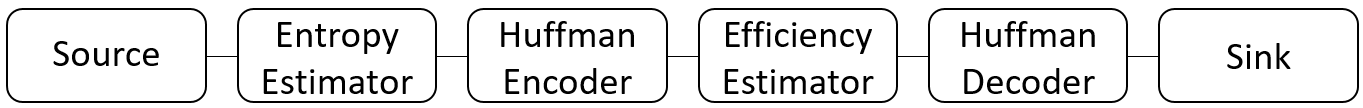
\includegraphics[width=6in]{./sdf/eit_45550_estimator_source_code_efficiency/figures/blockdiagram.png}
\caption[Block diagram of communication system]{Block diagram of source code efficiency implementation.}
\label{f:RF_C}
\end{figure}

In the following sections each block will be explained in detailed.


\subsubsection{Entropy Estimator}
In the Entropy Estimator block the main goal is to calculated the entropy from a binary source for the case of a binary source composed by 0 and 1. In this sense, to calculated the entropy the equation \ref{e:eq2} was applied.


\begin{equation}
H(x)=\sum_{i=1}^K P(a_{i})  \log_2\frac{1}{P(a_{i})}
 \label{e:eq2}
\end{equation}

This block does not have inputs variables.

\subsubsection{Hufmman Encoder}
The Hufman Encoder block aims to encode a binary signal, composed by 0 and 1, for a order of 2, 3 and 4. This block has 2 input variables, the probabilityOfZero and sourceOrder. 
The probabilityOfZero variable is a double value with a range from 0 until 1. The sourceOrder variable is a integer value, where only 2, 3 and 4 values are accepted.

In this Huffman encoder, the probabilityOfZero will defined the type of codification, as well as, the source order. For a probability of zero less or equal than a probability of one, the encoder process is presented in tables \ref{tb:hufmmanencoder2}, \ref{tb:hufmmanencoder4} and \ref{tb:hufmmanencoder6}, for a source order of 2, 3 and 4 respectively.
Otherwise, if probability of zero is greater than probability of one, the encoder process is shown in tables \ref{tb:hufmmanencoder3}, \ref{tb:hufmmanencoder5} and \ref{tb:hufmmanencoder7}, for a source order of 2, 3 and 4 respectively.

\begin{table}[H]
\centering
\caption{Huffman Encoder 2 Order, when probability of Zero less or equal than probability of One}
\label{tb:hufmmanencoder2}
\begin{tabular}{|l|l|l|}
\hline
\textbf{Message}                      & \textbf{Huffman Encoder Order 2}                                       \\ \hline
00                 & 111                                                          \\ \hline
01                 & 110                                                          \\ \hline
10                 & 10                                                         \\ \hline
10                 & 0                                                         \\ \hline

\end{tabular}
\end{table}

\begin{table}[H]
\centering
\caption{Huffman Encoder 2 Order, when probability of Zero greater than probability of One}
\label{tb:hufmmanencoder3}
\begin{tabular}{|l|l|l|}
\hline
\textbf{Message}                      & \textbf{Huffman Encoder Order 2}                                       \\ \hline
11                 & 111                                                          \\ \hline
10                 & 110                                                          \\ \hline
01                 & 10                                                         \\ \hline
00                 & 0                                                         \\ \hline

\end{tabular}
\end{table}


\begin{table}[H]
\centering
\caption{Huffman Encoder 3 Order, when probability of Zero less or equal than probability of One}
\label{tb:hufmmanencoder4}
\begin{tabular}{|l|l|l|}
\hline
\textbf{Message}                      & \textbf{Huffman Encoder Order 3}                                       \\ \hline
000                 & 1111111                                                          \\ \hline
001                 & 1111110                                                          \\ \hline
010                 & 111110                                                         \\ \hline
011                 & 11110                                                   \\ \hline
100                 & 1110                                                          \\ \hline
101                 & 110                                                          \\ \hline
110                 & 10                                                         \\ \hline
111                 & 0                                                         \\ \hline
\end{tabular}
\end{table}

\begin{table}[H]
\centering
\caption{Huffman Encoder 3 Order, when probability of Zero greater than probability of One}
\label{tb:hufmmanencoder5}
\begin{tabular}{|l|l|l|}
\hline
\textbf{Message}                      & \textbf{Huffman Encoder Order 3}                                       \\ \hline
111                 & 1111111                                                          \\ \hline
110                 & 1111110                                                          \\ \hline
101                 & 111110                                                         \\ \hline
100                 & 11110                                                   \\ \hline
011                 & 1110                                                          \\ \hline
010                 & 110                                                          \\ \hline
001                 & 10                                                         \\ \hline
000                 & 0                                                         \\ \hline
\end{tabular}
\end{table}



\begin{table}[H]
\centering
\caption{Huffman Encoder 4 Order, when probability of Zero less or equal than probability of One}
\label{tb:hufmmanencoder6}
\begin{tabular}{|l|l|l|}
\hline
\textbf{Message}                      & \textbf{Huffman Encoder Order 4}                                       \\ \hline
0000                 & 111111111111111                                                         \\ \hline
0001                 & 111111111111110                                              \\ \hline
0010                 & 11111111111110                                            \\ \hline
0011                 & 1111111111110                                       \\ \hline
0100                 & 111111111110                                                          \\ \hline
0101                 & 11111111110                                                          \\ \hline
0110                 & 1111111110                                                         \\ \hline
0111                 & 111111110                                                         \\ \hline
1000                 & 11111110                                                          \\ \hline
1001                 & 1111110                                                          \\ \hline
1010                 & 111110                                                         \\ \hline
1011                 & 11110                                                   \\ \hline
1100                 & 1110                                                          \\ \hline
1101                 & 110                                                          \\ \hline
1110                 & 10                                                         \\ \hline
1111                 & 0                                                         \\ \hline
\end{tabular}
\end{table}


\begin{table}[H]
\centering
\caption{Huffman Encoder 4 Order, when probability of Zero greater than probability of One}
\label{tb:hufmmanencoder7}
\begin{tabular}{|l|l|l|}
\hline
\textbf{Message}                      & \textbf{Huffman Encoder Order 4}                                       \\ \hline
1111                 & 111111111111111                                                         \\ \hline
1110                 & 111111111111110                                              \\ \hline
1101                 & 11111111111110                                            \\ \hline
1100                 & 1111111111110                                       \\ \hline
1011                 & 111111111110                                                          \\ \hline
1010                 & 11111111110                                                          \\ \hline
1001                 & 1111111110                                                         \\ \hline
1000                 & 111111110                                                         \\ \hline
0111                 & 11111110                                                          \\ \hline
0110                 & 1111110                                                          \\ \hline
0101                 & 111110                                                         \\ \hline
0100                 & 11110                                                   \\ \hline
0011                 & 1110                                                          \\ \hline
0010                 & 110                                                          \\ \hline
0001                 & 10                                                         \\ \hline
0000                 & 0                                                         \\ \hline
\end{tabular}
\end{table}

\subsubsection{Efficiency Estimator}
The Efficiency Estimator (Source Code Efficiency) block goal is to calculate the efficiency of the code, for a order code of 2, 3 and 4. This block has 2 input variables, the probabilityOfZero and sourceOrder.
In this sense, to calculate the efficiency, the equation \ref{e:eq} was used, where L is length codeword.

\begin{equation}
\eta=\frac{Hr(x)}{L}
 \label{e:eq}
\end{equation}

\subsubsection{Hufman Decoder}


The Hufman Decoder block aims to decode signal from Huffman Encoder block, composed by 0 and 1, for a order of 2, 3 and 4. This block has 2 input variables, the probabilityOfZero and sourceOrder. 
The probabilityOfZero variable is a double value with a range from 0 until 1. The sourceOrder variable is a integer value, where only 2, 3 and 4 are accepted.

In this Huffman decoder, the probabilityOfZero will defined the type of descodification, as well as, the source order. For a probability of zero less or equal than a probability of one, the decoder process is presented in tables \ref{tb:hufmmandecoder2}, \ref{tb:hufmmandecoder4} and \ref{tb:hufmmandecoder6}, for a source order of 2, 3 and 4 respectively.
Otherwise, if probability of zero is greater than probability of one, the decoder process is shown in tables \ref{tb:hufmmandecoder3}, \ref{tb:hufmmandecoder5} and \ref{tb:hufmmandecoder7}, for a source order of 2, 3 and 4 respectively.


\begin{table}[H]
\centering
\caption{Huffman Decoder 2 Order, when probability of Zero less or equal than probability of One}
\label{tb:hufmmandecoder2}
\begin{tabular}{|l|l|l|}
\hline
\textbf{Message}                      & \textbf{Huffman Decoder Order 2}                                       \\ \hline
111              & 00                                               \\ \hline
110              & 01                                           \\ \hline
10                & 10                                      \\ \hline
0                  & 11                                  \\ \hline

\end{tabular}
\end{table}

\begin{table}[H]
\centering
\caption{Huffman Decoder 2 Order, when probability of Zero greater than probability of One}
\label{tb:hufmmandecoder3}
\begin{tabular}{|l|l|l|}
\hline
\textbf{Message}                      & \textbf{Huffman Decoder Order 2}                                       \\ \hline
111         &11                                                          \\ \hline
110         &10                                                        \\ \hline
10           &01                                               \\ \hline
0             &00                                       \\ \hline

\end{tabular}
\end{table}


\begin{table}[H]
\centering
\caption{Huffman Decoder 3 Order, when probability of Zero less or equal than probability of One}
\label{tb:hufmmandecoder4}
\begin{tabular}{|l|l|l|}
\hline
\textbf{Message}                      & \textbf{Huffman Decoder Order 3}                                       \\ \hline
1111111    & 000                                                      \\ \hline
1111110    & 001                                                     \\ \hline
111110      & 010                                                   \\ \hline
11110        & 011                                          \\ \hline
1110          & 100                                               \\ \hline
110            & 101                                             \\ \hline
10              & 110                                          \\ \hline
0                & 111                                         \\ \hline
\end{tabular}
\end{table}

\begin{table}[H]
\centering
\caption{Huffman Decoder 3 Order, when probability of Zero greater than probability of One}
\label{tb:hufmmandecoder5}
\begin{tabular}{|l|l|l|}
\hline
\textbf{Message}                      & \textbf{Huffman Decoder Order 3}                                       \\ \hline
 1111111 &111                                                                           \\ \hline
1111110  &110                                                          \\ \hline
111110    &101                                                    \\ \hline
11110      &100                                              \\ \hline
1110        &011                                                  \\ \hline
110          &010                                                 \\ \hline
10            &001                                              \\ \hline
0              &000                                            \\ \hline
\end{tabular}
\end{table}



\begin{table}[H]
\centering
\caption{Huffman Decoder 4 Order, when probability of Zero less or equal than probability of One}
\label{tb:hufmmandecoder6}
\begin{tabular}{|l|l|l|}
\hline
\textbf{Message}                      & \textbf{Huffman Decoder Order 4}                                       \\ \hline
111111111111111         & 0000                                                \\ \hline
111111111111110         & 0001                                      \\ \hline
11111111111110           & 0010                                  \\ \hline
1111111111110             & 0011                          \\ \hline
111111111110               & 0100                                           \\ \hline
11111111110                 & 0101                                          \\ \hline
1111111110                   & 0110                                      \\ \hline
111111110                     & 0111                                    \\ \hline
11111110                       & 1000                                   \\ \hline
1111110                         & 1001                                 \\ \hline
111110                           & 1010                              \\ \hline
11110                             & 1011                      \\ \hline
1110                               & 1100                           \\ \hline
110                                 & 1101                         \\ \hline
10                                   & 1110                      \\ \hline
 0                                    & 1111                     \\ \hline
\end{tabular}
\end{table}


\begin{table}[H]
\centering
\caption{Huffman Decoder 4 Order, when probability of Zero greater than probability of One}
\label{tb:hufmmandecoder7}
\begin{tabular}{|l|l|l|}
\hline
\textbf{Message}                      & \textbf{Huffman Decoder Order 4}                                       \\ \hline
111111111111111      & 1111                                                   \\ \hline
111111111111110      & 1110                                        \\ \hline
11111111111110        & 1101                                    \\ \hline
1111111111110          & 1100                             \\ \hline
111111111110            & 1011                                              \\ \hline
11111111110              & 1010                                            \\ \hline
1111111110                & 1001                                         \\ \hline
111111110                  & 1000                                       \\ \hline
11111110                    & 0111                                      \\ \hline
1111110                      & 0110                                     \\ \hline
111110                        & 0101                                 \\ \hline
11110                          & 0100                         \\ \hline
1110                            & 0011                              \\ \hline
110                              & 0010                            \\ \hline
10                                & 0001                         \\ \hline
0                                  & 0000                      \\ \hline
\end{tabular}
\end{table}

In table \ref{tb:inputparameters2} are presented the input parameters of the system.





\subsection{Simulation Analysis}

The simulation implementation will be described in order to implement the Source Code Efficiency project. In Figure \ref{f:simulationdiagram} the block diagram of simulation process is shown.
For this simulation, the value of probabilityOfZero variable was 0.05. 

\begin{figure}[!h]
\centering
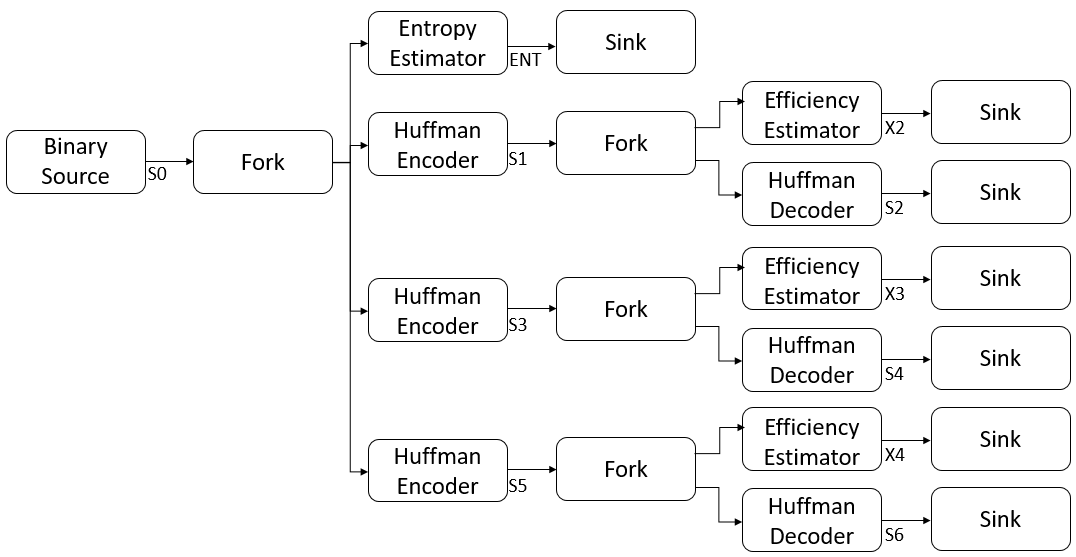
\includegraphics[width=6in]{./sdf/eit_45550_estimator_source_code_efficiency/figures/simulationdiagram.png}
\caption[Simulation Block diagram.]{Simulation Block diagram.}
\label{f:simulationdiagram}
\end{figure}

First, the Binary source block is executed, in order to generate a sequence of random binary bits, which results in the S0 signal. In Figure \ref{f:S0} can be seen an example of a S0 signal, as a result of Binary Source code. 


\begin{figure}[!h]
\centering
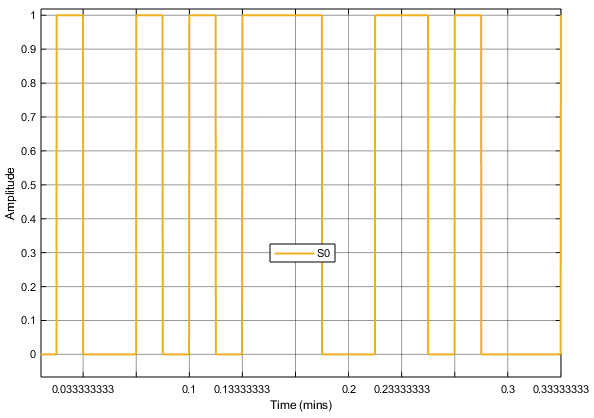
\includegraphics[width=5in]{./sdf/eit_45550_estimator_source_code_efficiency/figures/S0.png}
\caption[S0 Signal from binary source.]{S0 Signal from binary source.}
\label{f:S0}
\end{figure}

After acquired the S0 signal, a fork was made to copy this signal. Four copies were created, one copy of this signal was applied in Entropy Estimator block, other in Huffman Encoder 2 order,  other in Huffman Encoder 3 order and the last copy was applied in Huffman Encoder 4 order.

The first copy was applied to Entropy Estimator block to estimate the entropy value of this random binary code, the resulting entropy signal from this block is shown in Figure \ref{f:entropy}. As expected, the entropy value converges to 1.
\begin{figure}[!h]
\centering
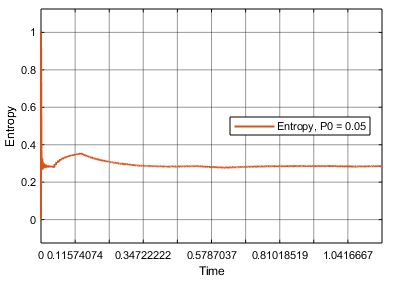
\includegraphics[width=4in]{./sdf/eit_45550_estimator_source_code_efficiency/figures/entropy.png}
\caption[Entropy results for aa binary source.]{Entropy results for a binary source.  The entropy theorical value is 0.2864.}
\label{f:entropy}
\end{figure}

The second copy was applied in the Hufman Encoder, with a source order of 2. In Figure \ref{f:S1} is presented the S1 signal, which is the result of Hufman Encoder 2 order, when the S0 signal was encoded.
Then, a fork was applied to copy the signal S1 in 2 signals, one to applied in the Efficiency Estimator block and other to applied in the Hufman Decoder block, using a source order of 2.
From the Efficiency Estimator arises the signal X2, wich can be seen in Figure \ref{f:efficiencygraph} and the decoder signal S2 from Hufman Decoder block, for a order of 2 appears in Figure \ref{f:S2}. 
\begin{figure}[!h]
\centering
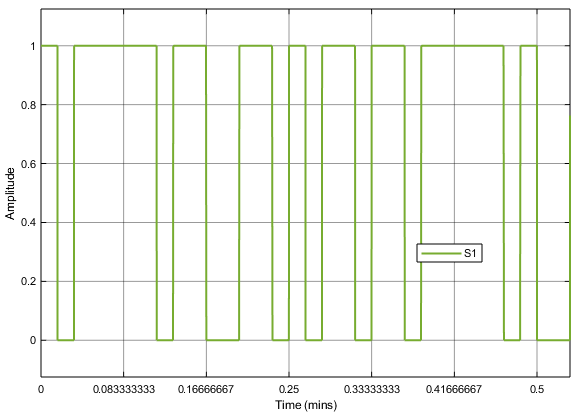
\includegraphics[width=5in]{./sdf/eit_45550_estimator_source_code_efficiency/figures/S1.png}
\caption[S1 Signal from Hufman Encoder 2 order.]{S1 Signal from Hufman Encoder 2 order.}
\label{f:S1}
\end{figure}


\begin{figure}[!h]
\centering
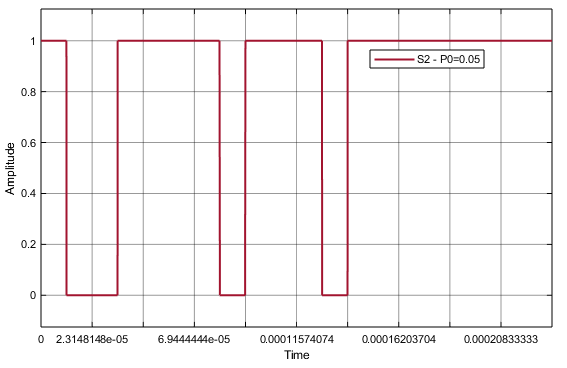
\includegraphics[width=5in]{./sdf/eit_45550_estimator_source_code_efficiency/figures/S2.png}
\caption[S2 Signal from Hufman Decoder 2 order.]{S2 Signal from Hufman Decoder 2 order.}
\label{f:S2}
\end{figure}

The third copy of signal S0 was applied in the Hufman Encoder, with a source order of 3. In Figure \ref{f:S3} is presented the S3 signal, which is the result of Hufman Encoder 3 order, when the S0 signal was encoded.
Then, a fork was applied to copy the signal S3 in 2 signals, one to applied in the Efficiency Estimator block and other to applied in the Hufman Decoder block, using a source order of 3.
From the Efficiency Estimator arises the signal X3, wich can be seen in Figure \ref{f:efficiencygraph} and the decoder signal S4 from Hufman Decoder block, for a order of 3 appears in Figure \ref{f:S4}. 

\begin{figure}[!h]
\centering
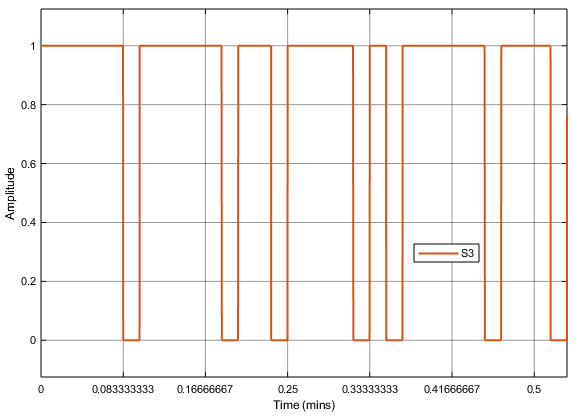
\includegraphics[width=5in]{./sdf/eit_45550_estimator_source_code_efficiency/figures/S3.png}
\caption[S3 Signal from Hufman Encoder 3 order.]{S3 Signal from Hufman Encoder 3 order.}
\label{f:S3}
\end{figure}


\begin{figure}[!h]
\centering
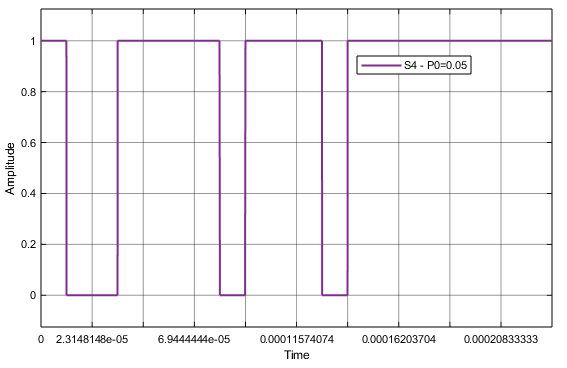
\includegraphics[width=5in]{./sdf/eit_45550_estimator_source_code_efficiency/figures/S4.png}
\caption[S4 Signal from Hufman Decoder 3 order.]{S4 Signal from Hufman Decoder 3 order.}
\label{f:S4}
\end{figure}

The fourth copy of signal S0 was applied in the Hufman Encoder, with a source order of 4. In Figure \ref{f:S5} is presented the S5 signal, which is the result of Hufman Encoder 4 order, when the S0 signal was encoded.
Then, a fork was applied to copy the signal S5 in 2 signals, one to applied in the Efficiency Estimator block and other to applied in the Hufman Decoder block, using a source order of 4.
From the Efficiency Estimator arises the signal X4, wich can be seen in Figure \ref{f:efficiencygraph} and the decoder signal S6 from Hufman Decoder block, for a order of 4 appears in Figure \ref{f:S6}. 


\begin{figure}[!h]
\centering
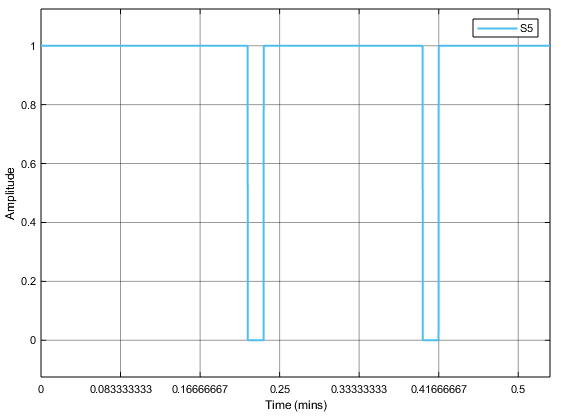
\includegraphics[width=5in]{./sdf/eit_45550_estimator_source_code_efficiency/figures/S5.png}
\caption[S5 Signal from Hufman Encoder 4 order.]{S5 Signal from Hufman Encoder 4 order.}
\label{f:S5}
\end{figure}


\begin{figure}[!h]
\centering
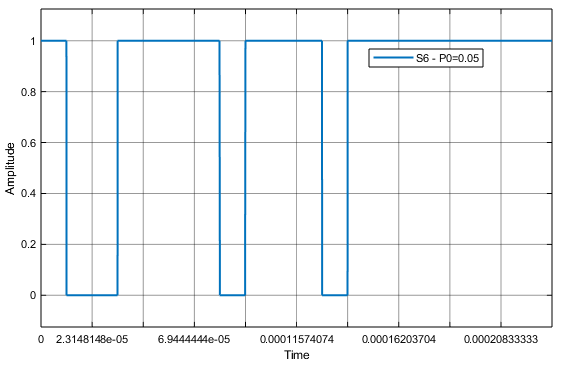
\includegraphics[width=5in]{./sdf/eit_45550_estimator_source_code_efficiency/figures/S6.png}
\caption[S6 Signal from Hufman Decoder 4 order.]{S6 Signal from Hufman Decoder 4 order.}
\label{f:S6}
\end{figure}

In order to validate that the encoder and decoder Hufman process was well developed for 2, 3 and 4 order, the original signal S0 was compared with signals S2, S4 and S6, which are the decoded signals of a source order of 2, 3 and 4 respectively.
This comparation of signals can be seen in Figure \ref{f:S0S2S4S6}. As can be seen, the signals are overlapping, which proves that the coding and decoding process were well applied.

\begin{figure}[!h]
\centering
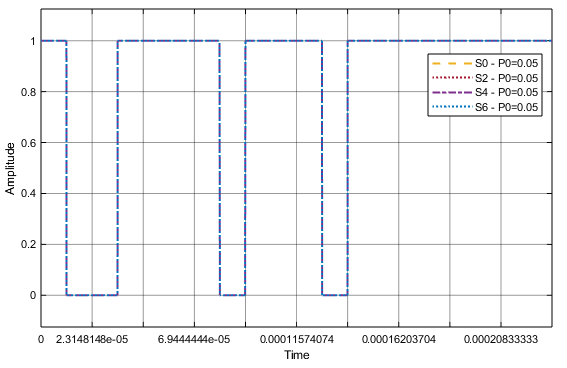
\includegraphics[width=5in]{./sdf/eit_45550_estimator_source_code_efficiency/figures/S0S2S4S6.png}
\caption[S0, S2, S4 and S6 signals comparation]{S0, S2, S4 and S6 signals comparation.}
\label{f:S0S2S4S6}
\end{figure}

In Figure \ref{f:efficiencygraph} can be seen the efficiency results for a source order of 2, 3 and 4 respectively. As expected, when the source order increases, the efficiency of the code decreases.

\begin{figure}[!h]
\centering
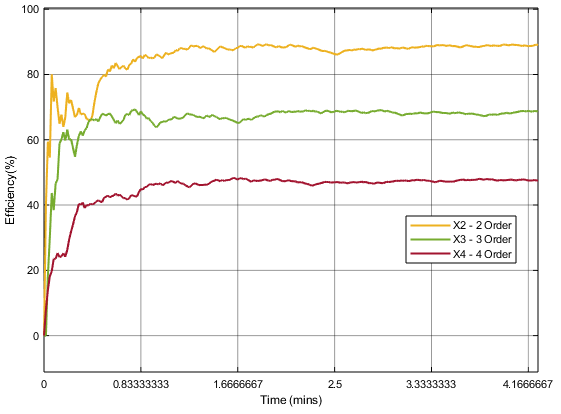
\includegraphics[width=4.2in]{./sdf/eit_45550_estimator_source_code_efficiency/figures/efficiencygraph.png}
\caption[Efficiency results for 2, 3 and 4 orders using Hufman Encoder.]{Efficiency results for 2, 3 and 4 orders using Hufman Encoder. The efficiency theorical values for each order are 49.92\%, 63.65\% and 65.46\%, respectively.}
\label{f:efficiencygraph}
\end{figure}

In the end, the sink block was used to to empty the buffer.

The project is composed by several parts. Table \ref{tb:signalsh2} shows the header files used to implement the simulation presented in Figure \ref{f:simulationdiagram}.
The source files are presented in table \ref{tb:signalss} and finally, in table \ref{tb:signals22} are shown the system signals, with the signal type information and description.
\begin{table}[H]
\centering
\caption{Header Files}
\label{tb:signalsh2}
\begin{tabular}{|c|c|c|}
\hline
\textbf{File name}                              & \textbf{Description}                                                          & \textbf{Status} \\ \hline
binary\_source\_20180523.h              &                      &    \checkmark   \\ \hline
entropy\_estimator\_20180621.h                           &                      &    \checkmark   \\ \hline
fork\_20180112.h      &                      &   \checkmark   \\ \hline
huffman\_decoder\_20180621.h                         &                      &    \checkmark   \\ \hline
huffman\_encoder\_20180621.h          &                      &    \checkmark   \\ \hline
netxpto\_20180418.h           &                      &    \checkmark   \\ \hline
sink\_20180118.h            &                      &    \checkmark   \\ \hline
source\_code\_efficiency\_20180621.h                                    &                      &    \checkmark   \\ \hline
\end{tabular}
\end{table}

\begin{table}[H]
\centering
\caption{Source Files}
\label{tb:signalss}
\begin{tabular}{|c|c|c|}
\hline
\textbf{File name}                              & \textbf{Description} & \textbf{Status} \\ \hline
binary\_source\_20180523.cpp              &                      &    \checkmark   \\ \hline
eit\_45550\_estimator\_source\_code\_efficiency\_sdf.cpp     &                      &    \checkmark   \\ \hline
entropy\_estimator\_20180621.cpp                             &                      &    \checkmark   \\ \hline
fork\_20180112.cpp      &                      &   \checkmark   \\ \hline
huffman\_decoder\_20180621.cpp                         &                      &    \checkmark   \\ \hline
huffman\_encoder\_20180621.cpp          &                      &    \checkmark   \\ \hline
netxpto\_20180418.cpp            &                      &    \checkmark   \\ \hline
sink\_20180118.cpp            &                      &    \checkmark   \\ \hline
source\_code\_efficiency\_20180621.cpp                                        &                      &    \checkmark   \\ \hline
\end{tabular}
\end{table}


\begin{table}[h]
\centering
\caption{System Signals}
\label{tb:signals22}
\begin{tabular}{|c|c|c|}
\hline
\textbf{Signal name}                            & \textbf{Signal type}         & \textbf{Description}                   \\ \hline

S0                                              &  Binary    & Binary signal which results \\
 &&from Source block\\ 
\hline

ENT                                              &  TimeContinuousAmplitudeContinuousReal  &  Entropy signal which results \\ 
 &&from Entropy Estimator block\\ 
\hline

S1                                              &  Binary                          & Signal encoded by Huffman\\ 
 && Encoder block, with order 2\\ 
\hline
X2                                              &  TimeContinuousAmplitudeContinuousReal   &Efficiency signal which results from                 \\
 &&Source Code Efficiency block\\ 
 && with order 2\\ 
 \hline
S2                                              &  Binary                        & Binary signal decoder by Huffman\\ 
 &&  Decoder block, with order 2\\ 
\hline
S3                                              &  Binary    &Signal encoded by Huffman\\ 
 && Encoder block, with order 3\\ 
\hline
X3                                              &  TimeContinuousAmplitudeContinuousReal &   Efficiency signal which results from                 \\
 &&Source Code Efficiency block\\ 
 && with order 3\\ 
 \hline
S4                                              &  Binary                                   & Binary signal decoder by Huffman\\ 
 &&  Decoder block, with order 3\\ 
\hline
S5                                              &  Binary    &Signal encoded by Huffman\\ 
 && Encoder block, with order 4\\ 
\hline
X4                                              &  TimeContinuousAmplitudeContinuousReal &   Efficiency signal which results from                 \\
 &&Source Code Efficiency block\\ 
 && with order 4\\ 
 \hline
S6                                              &  Binary                                   & Binary signal decoder by Huffman\\ 
 &&  Decoder block, with order 4\\ 
\hline
\end{tabular}
\end{table}

To run this simulation, different values can be applied to the probabilityOfZero variable.


% bibliographic references for the section ----------------------------
\clearpage
%\printbibliography[heading=subbibliography]
\end{refsection}
%\addcontentsline{toc}{subsection}{Bibliography}
\cleardoublepage
% --------------------------------------------------------------------- 